\documentclass{article}
\usepackage[utf8]{inputenc}
\usepackage[T1]{fontenc}
\usepackage[french]{babel}
\usepackage{graphicx}

\title{Rendu n.1 Projet technologique}
\author{Zoé Debaty}
\date{November 2019}

\begin{document}

\maketitle
\tableofcontents 
\newpage

% Spécificités techniques %
\section{Spécificités techniques}

% L'image %
\subsection{L'image}
\begin{center} 
    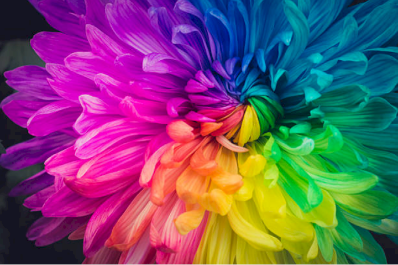
\includegraphics[width=9cm]{../multicolor}
    \end{center}

\begin{itemize}
\item Nom : "multicolor"
\item Dimensions : 612p * 408p
\item Taille : 59,9 Ko
\end{itemize}
\medbreak

L'image à été choisie car elle possède des changements de luminosité et énorméments de couleurs afin de tester au mieux mes fonctions.
C'est la seule image sur laquelle les fonctions ont été testées pour l'instant.

% Le telephone %
\subsection{Le téléphone}
Pour tester mes fonctions j'utilise un Sony Xpéria XA, avec une définition d'écran de 1280 * 720 et une diagonale de 5 pouces.\\
Il tourne sous Android Nougat 7.0.
\newpage

% Functions %
\section{Fonctions}

% Saturation %
\subsection{Saturation}
Cette fonction permet de modifier la saturation de l'image en ajoutant / enlevant des pourcentages (10\%) à l'image HSV.
\bigbreak

\begin{center} 
    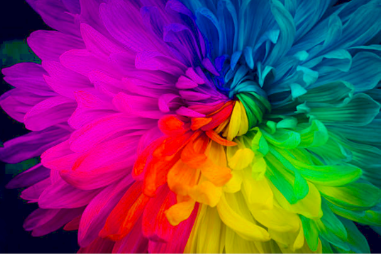
\includegraphics[width=9cm]{../SaturationMax}

    Image de base avec la saturation au maximum.
    \end{center}
\bigbreak

\begin{center} 
    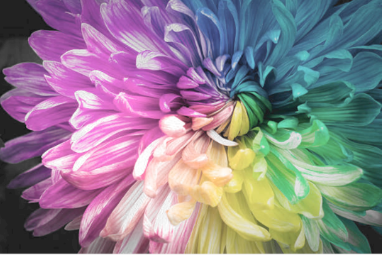
\includegraphics[width=9cm]{../SaturationMoins6}

    Image de base avec 60\% de saturation en moins.
    \end{center}

% Luminosite %
\subsection{Luminosité}
Cette fonction permet de changer la luminosité de l'image en ajoutant / enlevant des pourcentages (10\%) à l'image HSV.
\bigbreak

\begin{center} 
    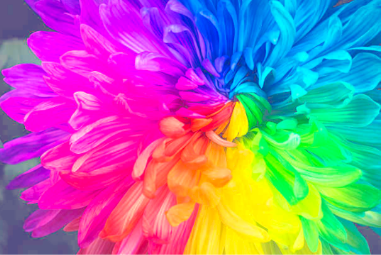
\includegraphics[width=9cm]{../LuminositePlus3}

    Image de base avec 30\% de luminosité en plus.
    \end{center}
\bigbreak

\begin{center} 
    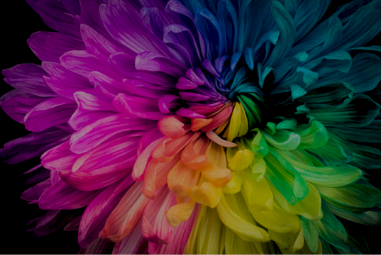
\includegraphics[width=9cm]{../LuminositeMoins3}

    Image de base avec 30\% de luminosité en moins.
    \end{center}

% Selection de couleurs %
\subsection{Selection de couleurs \underline{TD 2 Qestion 2.2}}
Cette fonction permet, au moyen de deux limites (qu'on modifie de 10 en 10), d'afficher ou non certaines couleurs.
\bigbreak

\begin{center} 
    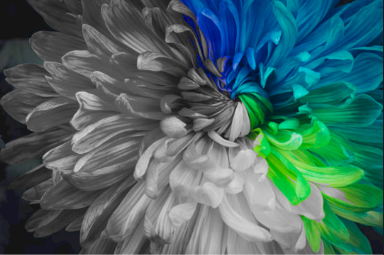
\includegraphics[width=9cm]{../SelectedColor}

    Image de base avec les deux limites n'affichants que les parties bleus et vertes de l'image.
    \end{center}

% Negatif %
\subsection{Negatif}
Cette fonction passe l'image en négatif.
\bigbreak

\begin{center} 
    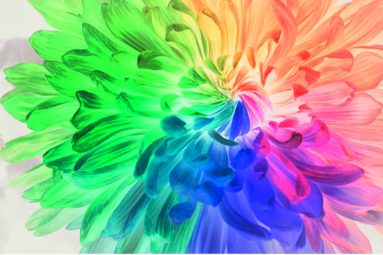
\includegraphics[width=9cm]{../Negatif}

    Image de base en négatif
    \end{center}

\begin{center} 
    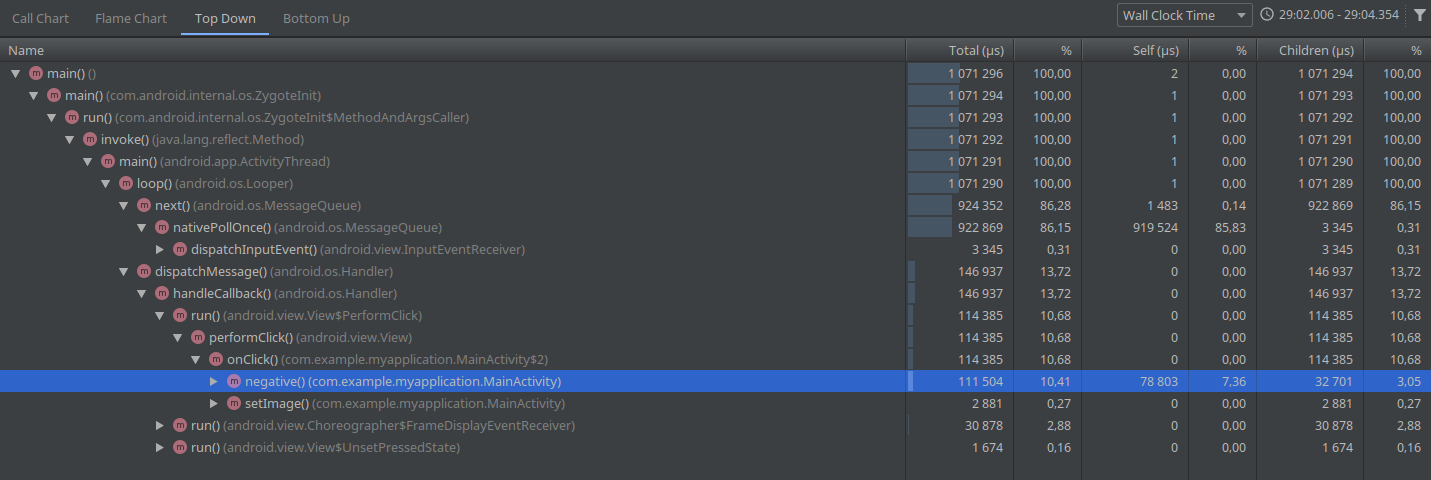
\includegraphics[width=11cm]{../TempsNegative}

    Temps de traitement de la fonction negative()
    \end{center}

% Version grise %
\subsection{Version grise \underline{TD 1 Question 3}}
Cette fonction grise l'image.
\bigbreak

\begin{center} 
    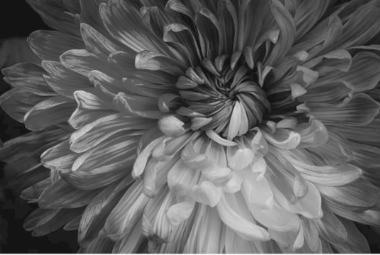
\includegraphics[width=9cm]{../Gris}

    Image de base grisée
    \end{center}
\bigbreak

\begin{center} 
    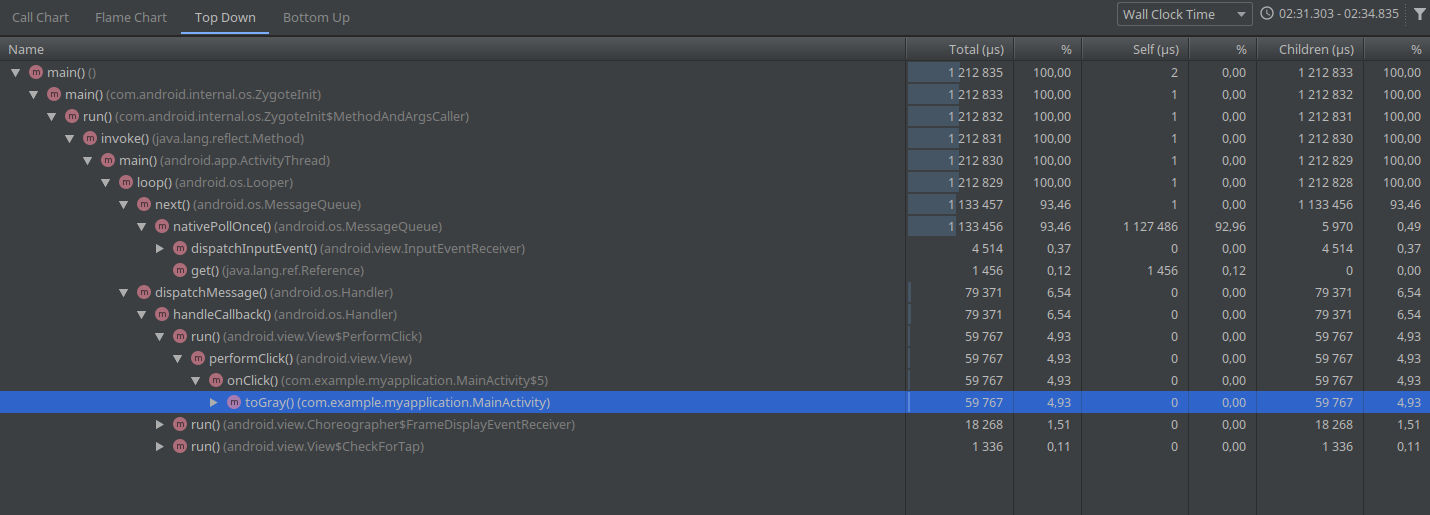
\includegraphics[width=11cm]{../TempsToGray}

    Temps de traitement de la fonction ToGray()
    \end{center}

% Extension linéaire %
\subsection{Extension linéaire \underline{TD 3 Qestion 1.1}}
Cette fonction est l'implémentation de l'augmentation du contraste par extension de dynamique.
\bigbreak

\begin{center} 
    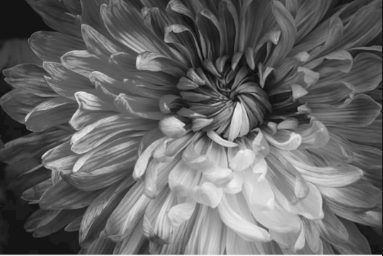
\includegraphics[width=9cm]{../ExtensionLineaire}

    Image de base grisée puis modifiée avec l'extension linéaire.
    \end{center}

\begin{center} 
    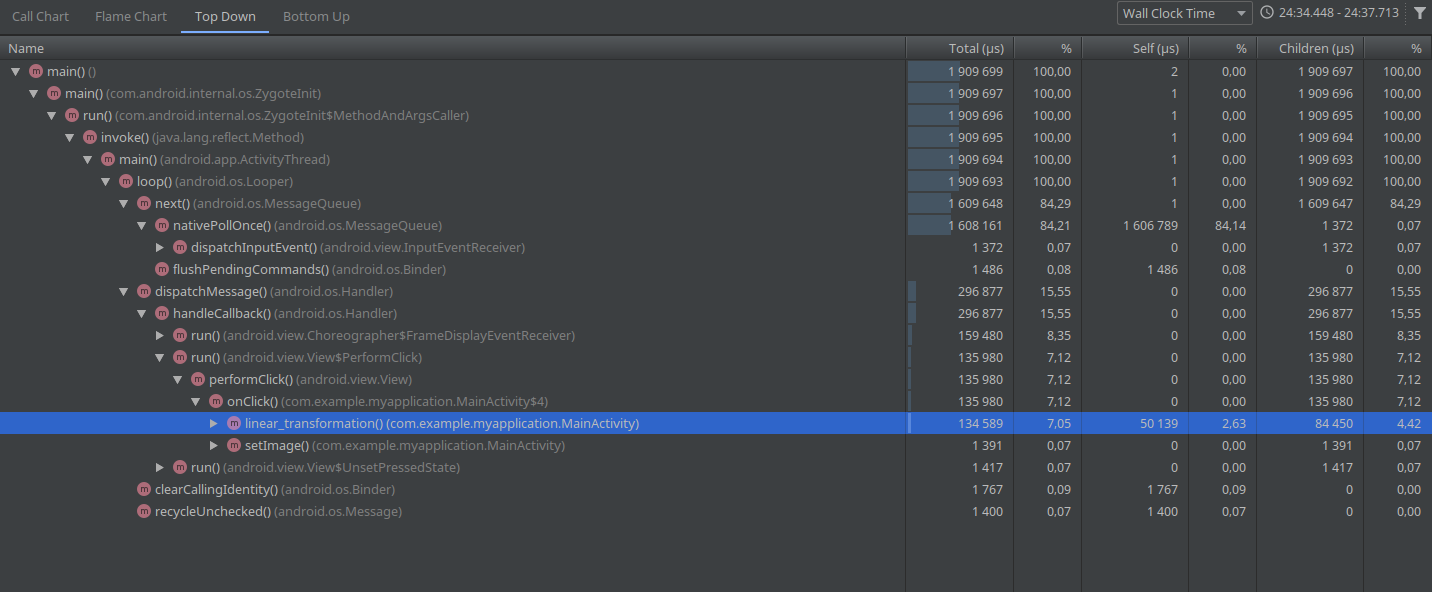
\includegraphics[width=11cm]{../TempsLinearTransformation}

    Temps de traitement de la fonction linear\_transformation()
    \end{center}

% Couleur aleatoire %
\subsection{Couleur aléatoire \underline{TD 2 Question 2.1}}
Cette fonction permet de coloriser l'image avec une couleur choisie aléatoirement.
\bigbreak

\begin{center} 
    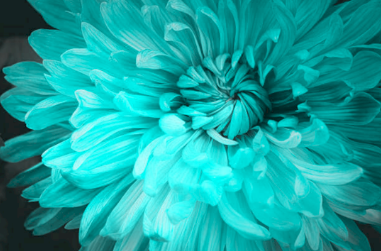
\includegraphics[width=9cm]{../RandomCouleur1}

    Image colorisé avec une couleur aléatoire (exemple 1)
    \end{center}
\bigbreak

\begin{center} 
    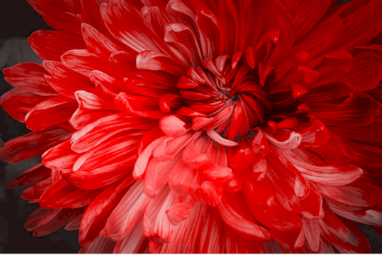
\includegraphics[width=9cm]{../RandomCouleur2}

    Image colorisé avec une couleur aléatoire (exemple 2)
    \end{center}

\end{document}